\documentclass[a4paper,12pt]{article} % тип документа

% Поля страниц
\usepackage[left=2.5cm,right=2.5cm,
    top=2cm,bottom=2cm,bindingoffset=0cm]{geometry}
    
%Пакет дял таблиц   
\usepackage{multirow} 
    
%Отступ после заголовка    
\usepackage{indentfirst}


% Рисунки
\usepackage{floatrow,graphicx,calc}
\usepackage{wrapfig}

%%% Работа с картинками
\usepackage{graphicx}  % Для вставки рисунков
\graphicspath{{images/}{images2/}}  % папки с картинками
\setlength\fboxsep{3pt} % Отступ рамки \fbox{} от рисунка
\setlength\fboxrule{1pt} % Толщина линий рамки \fbox{}
\usepackage{wrapfig} % Обтекание рисунков и таблиц текстом

% Создаёем новый разделитель
\DeclareFloatSeparators{mysep}{\hspace{1cm}}

% Ссылки?
\usepackage{hyperref}
\usepackage[rgb]{xcolor}
\hypersetup{				% Гиперссылки
    colorlinks=true,       	% false: ссылки в рамках
	urlcolor=blue          % на URL
}


%  Русский язык
\usepackage[T2A]{fontenc}			% кодировка
\usepackage[utf8]{inputenc}			% кодировка исходного текста
\usepackage[english,russian]{babel}	% локализация и переносы

% Математика
\usepackage{amsmath,amsfonts,amssymb,amsthm,mathtools}

%%% Дополнительная работа с математикой
\usepackage{amsmath,amsfonts,amssymb,amsthm,mathtools} % AMS
\usepackage{icomma} % "Умная" запятая: $0,2$ $-$- число, $0, 2$ $-$- перечисление


% Что-то 
\usepackage{wasysym}


\begin{document}
\begin{center}
	\footnotesize{МОСКОВСКИЙ ФИЗИКО-ТЕХНИЧЕСКИЙ ИНСТИТУТ\\(НАЦИОНАЛЬНЫЙ 			ИССЛЕДОВАТЕЛЬСКИЙ УНИВЕРСИТЕТ)}\\
	\footnotesize{ФИЗТЕХ-ШКОЛА РАДИОТЕХНИКИ И КОМПЬЮТЕРНЫХ ТЕХНОЛОГИЙ\\}
	\hfill \break
	\hfill \break
	\hfill \break
	\hfill \break
	\hfill \break
	\hfill \break
\end{center}

\begin{center}   
    \hfill \break
	\hfill \break
	\hfill \break
	\hfill \break
	\hfill \break
	\hfill \break
	\hfill \break
	\hfill \break
	\hfill \break
	\hfill \break
	\hfill \break
	\large{Лабораторная работа № 4.3.2\\\large{\textbf{Дифракция света на ультразвуковой волне в жидкости}}}\\
	\hfill \break
        \hfill \break
	\hfill \break
	\hfill \break
	\hfill \break
	\hfill \break
	\hfill \break
	\hfill \break
	\hfill \break
	\hfill \break
	\hfill \break
	\begin{flushright}
		Климова Екатерина\\
		Группа Б01-108
	\end{flushright}
	\hfill \break
\end{center}
\hfill \break
\hfill \break
\begin{center}
	Долгопрудный, 2023 г.
\end{center}
\thispagestyle{empty}

\newpage
\hfill \break
\textbf{Цель работы:} изучение дифракции света на синусоидальной акустической решетке и наблюдение фазовой решетки методом темного поля.
\hfill \break
\hfill \break
\textbf{В работе используются:} оптическая скамья; осветитель; светофильтры; конденсор; щель; два длиннофокусных объектива; кювета с водой; кварцевый излучатель с микрометрическим винтом; генератор ультразвуковой частоты; частотомер; линза; отсчетное устройство; микроскоп.

\section{Аннотация}
\hfill \break В работе предлагается измерить координаты дифракционных полос, образующихся при дифракции света на акустической решетке, а также определить период этой решетки методом темного поля. По результатам измерений рассчитывается скорость ультразвука в воде. Все измерения ведутся на стоячей волне.

\section{Теоретические сведения}
\hfill \break В работе изучается дифракция света на фазовой решетке. Фазовая решетка создается в жидкости ультразвуковыми волнами и наблюдается методом темного поля.

\begin{wrapfigure}{l}{0.25\textwidth}
\begin{center}
    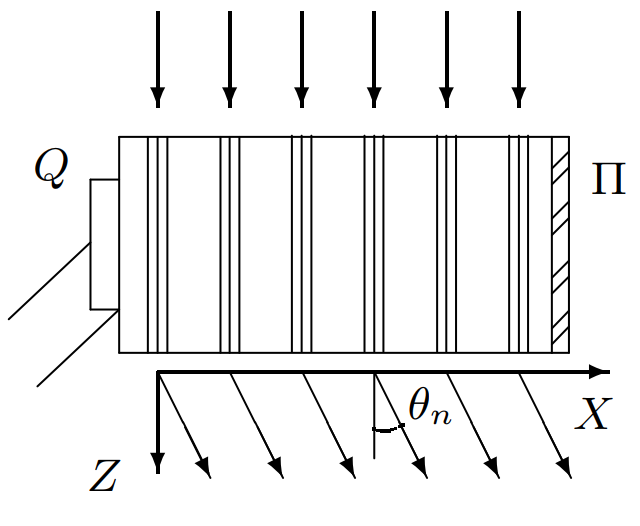
\includegraphics[width=1\textwidth]{4.3.2_1.png}
    \textbf{Рис. 1.} Дифракция световых волн на акустической решетке
\end{center}
\end{wrapfigure}

\hfill \break При прохождении ультразвуковой (УЗ) волны через жидкость в ней возникают периодические оптические неоднородности, обусловленные разницей значений коэффициента преломления в областях сжатия и разрежения. Эти периодические неоднородности играют роль своеобразной дифракционной решетки для прохзодящего сквозь жидкость света.

\hfill \break Пусть УЗ-волна распространяется вдоль оси $X$ (рис. 1) в жидкости, налитой в стеклянную кювету. В направлении оси $Z$ сквозь жидкость проходит световая волна, испытывающая дифракцию на акустической решетке. Поскольку скорость света значительно больше скорости звука, акустическую решетку можно считать неподвижной. Вызванное ультразвуком возмущение показателя преломления жидкости в нашем случае очень мало. При этом естественно сделать предположение, что акустическую решетку можно рассматривать как тонкий фазовый экран.

\hfill \break При небольших амплитудах звуковой волны показательб преломления жидкости $n$ меняется по закону

\begin{equation}\label{ linkname }
n = n_{0}(1 + m\cos{\Omega x}),
\end{equation}

\hfill \break где $\Omega$ $-$ волновое число для УЗ-волны $(\Omega = 2\pi/\Lambda)$, $\Lambda$ $-$ длина УЗ-волны, $m$ $-$ глубина модуляции показателя преломления, определяемая интенсивностью ультразвуковой волны ($m \ll 1)$.

\hfill \break Пусть фаза световых колебаний на передней поверхности жидкости равна нулю. Тогда на задней поверхности (т. е. в плоскости $z = 0$) она равна

\begin{equation}\label{ linkname }
\varphi = knL = \varphi_{0}(1 + m\cos{\Omega x},
\end{equation}

\hfill \break где $L$ $-$ толщина слоя жидкости в кювете, $k$ $-$ волновое число для света ($k = 2\pi/\lambda$), $\lambda$ $-$ длина световой волны, $\varphi_{0} = kn_{0}L$. Таким образом, в плоскости $z = 0$ фаза световых колебаний является периодической функцией координаты $x$, иными словами $-$ УЗ-волна в жидкости создает фазовую дифракционную решетку.

\hfill \break Можно сформулировать качественный критерий, при выполнении которого можно считать акустическую решетку чисто фазовой, то есть рассматривать ее как тонкий фазовый экран. Для нашей задачи условие тонкого транспаранта можно записать в виде

\begin{equation}\label{ linkname }
m \ll \frac {\Lambda} {L} \sqrt{ \frac {\lambda} {L} }.
\end{equation}

\hfill \break Таким образом, чисто фазовая акустическая решетка реализуется лишь на достаточно слабой УЗ-волне. При повышении мощности ультразвука акустическая волна начинает работать как мложная амплитудно-фазовая решетка.

\hfill \break После прохождения через кювету световое поле представляет совокупность не трех, а большого числа плоских волн, распространяющихся под углами, определяемыми условием

\begin{equation}\label{ linkname }
\Lambda \sin{\Theta_{m}} = m\lambda \text{ } (m = 0, \text{ } \pm 1, \text{ } \pm 2, \text{ } ...).
\end{equation}

\hfill \break Каждая из этих волн соответсует одному из максимумов в дифракционной картине Фраунгофера.

\hfill \break Определяя на опыте положение дифракционных максимумов различного порядка, можно по формуле (4) найти длину $\Lambda$ УЗ-волны и вычислить скорость $v$ распространения ультразвуковых волн в жидкости, если известна частота $\nu$ колебаний кварцевого излучателя:

\begin{equation}\label{ linkname }
v = \Lambda \nu.
\end{equation}

\hfill \break Рассматриваемая теория применима как для бегущих, так и для стоячиъ ультразвуковых волн. Стоячие УЗ-волны образуются при наложении волны, идущей от излучателя, и волны, отраженной от задней стенки кюветы. Если же заднюю стенку кюветы покрыть слоем пористой резины (слой П на рис. 1), то волна от нее не отражается и в кювете образуется практически чистая бегущая волна. Следует иметь в виду, что в стоячей волне амплитуда изменения давления (а следовательно, и коэффициента преломления) больше, чем в бегущей волне, создаваемой тем же излучателем. В связи с этим дифракционная картина в первом случае содержит большее число максимумов.

\section{Экспериментальная установка}
\subsection{Наблюдение дифракции на аустической решетке}
\hfill \break Экспериментальная установка для наблюдения дифракции света на УЗ-волнах изображена на рис. 2:

\begin{center}
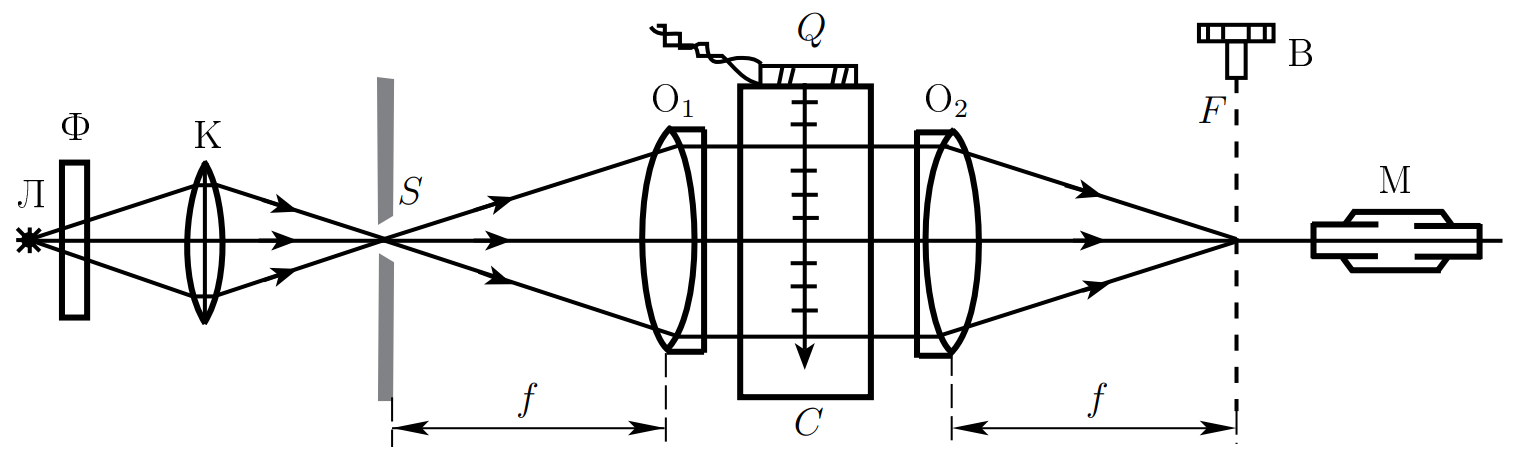
\includegraphics[width=0.75\textwidth]{4.3.2_2.png}\\
\textbf{Рис. 2.} Схема наблюдения дифракции на акустической решетке \\
\end{center}

\hfill \break Источник света Л через светофильтр Ф и конденсор К освещает щель $S$, которая расположена в фокусе объектива $O_{1}$. Выходящий из объектива параллельный пучок света проходит через кювету $C$ перпендикулярно направлению распространения УЗ-волн. Эти волны возбуждаются в жидкости пьезокварцевой пластинкой $Q$, прикрпеленной к стенке кюветы. На кварцевую пластинку подается синусоидальное направжение ультразвуковой частоты от генератора (на рис. 2 не показан). В результате взаимодействия света с ультразвуковой волной в фокальной плоскости второго объектива $O_2$ образуется дифракционная картина, наблюдаемая при помощи микроскопа $M$. При этом обяхательно применяют монохроматическое излучение (красный светофильтр).

\begin{wrapfigure}{r}{0.25\textwidth}
\begin{center}
    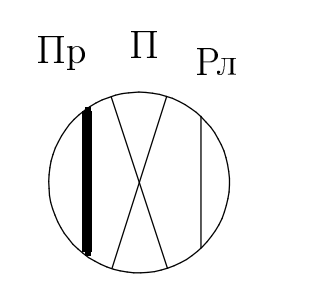
\includegraphics[width=1\textwidth]{4.3.2_3.png}
    \textbf{Рис. 3.} Проволока Пр, перекрестие П и реперная линия Рл на стекле отсчетного устройства
\end{center}
\end{wrapfigure}

\hfill \break Дифракционные полосы ориентированы вертикально. Расстояние между ними можно измерить с помощью специального отсчетного устройства с микрометрическим  винтом В. Этот винт передвигает размещенные на стекле отсчетного устройства (рис. 3) тонкую реперную линию Рл, перекрестие П и толстую проволоку Пр, которая используется в методе темного поля. Все измерительные линии должны быть расположены в плоскости $F$ резкого изображения щели.

\hfill \break Четкость дифракционных полос зависит от ряда факторов, например, от ширины щели $S$, от ее наклона по отношению к вертикали, от угла наклона кюветы к падающему лучу и т. д.

\hfill \break Длина $\Lambda$ УЗ-волны определяется по формуле (4):

$$
\Lambda \sin{\Theta_{m}} = m\lambda;
$$

\hfill \break в силу малости углов $\Theta_{m}$ окончательное выражение может быть представлена в виде

\begin{equation}\label{ linkname }
l_{m} = mf \frac{\lambda} {\Lambda},
\end{equation}

\hfill \break где $l_{m}$ $-$ измеренное на опыте линейное расстояние между $m$-м и нулевым максимумами, а $f$ $-$ фокусное расстояние объектива $O_{2}$.

\hfill \break Скорость $v$ распространения звука в воде можно считать, если известна частота $\nu$ кварцевого излучателя: $ v = \Lambda \nu $.

\subsection{Наблюдение оптических неоднородностей, создаваемых ультразвуковыми волнами в жидкости методом темного поля}
\hfill \break Попробуем теперь получить видимое изображение фазовой акустической решетки. Для этого прежде всего необходимо получить в поле зрения микроскопа изображение задней плоскости (считая по хожу световых лучей) кюветиы. Это достигается с помощью вспомогательной положительной линзы $O$, которую располагают на оптической скамье за фокальной плоскостью объектива $O_{2}$ (рис. 4).

\begin{center}
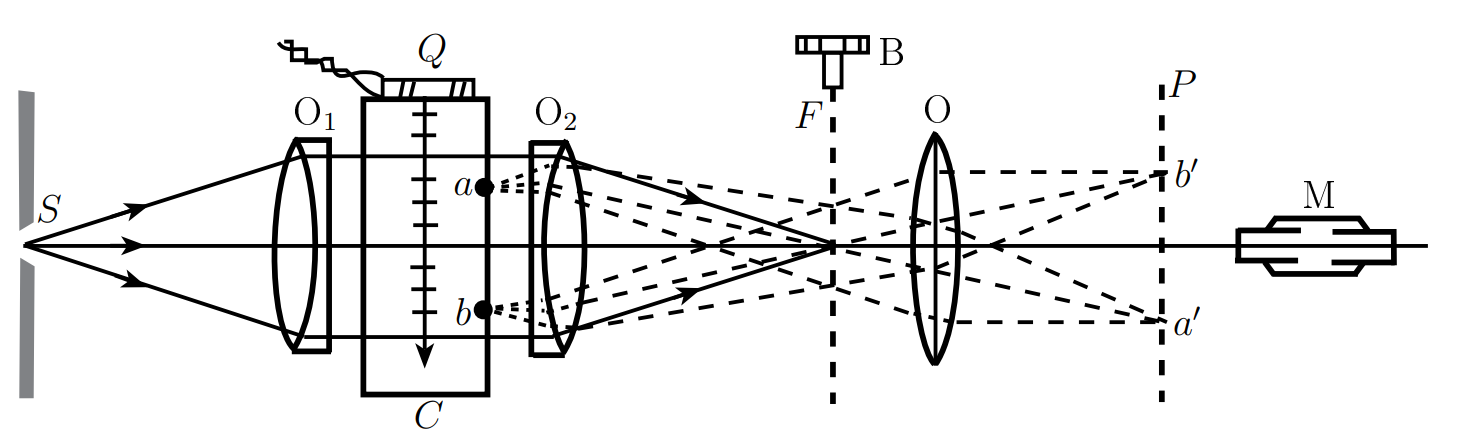
\includegraphics[width=0.75\textwidth]{4.3.2_4.png}\\
\textbf{Рис. 4.} Схема наблюдения акустической решетки методом темного поля \\
\end{center}

\hfill \break Перемещая микроскоп вдоль оптической скамьи, фокусируют его на плоскость $P$, где расположено четкое изображение $a'b'$ какого-либо предмета $ab$, вплотную прижатого к стенке кюветы. Можно ли теперь увидеть в микроскоп акустическую решетку $-$ УЗ-волну? Ясно, что чисто фазовая решетка является невидимой, если, конечно, выполнено условие (3): $m \ll \frac {\Lambda} {L} \sqrt{ {\lambda} {L} }$.

\hfill \break Для наблюдения акустической решетки в работе используется \textit{метод темного поля}, основанный на устранении центрального дифракционного максимума с помощью спецаильного экрана (проволочки). В центре экрана микроскопа наблюдаются чередующиеся светлые и темные полосы, причем расстояние между темными полосами соответсвует смещению и плоскости кюветы на $\Lambda/2$. Таким образом, наблюдается характерное для метода темного поля удвоение числа деталей рассматриваемой структуры. Картина интенсивности имеет вид:

$$
I(x) = m^2\cos^2{\Omega x}.
$$

\hfill \break Этот опыт можно проводить только со стоячими волнами, так как в случае бегущей волны визуальное наблюдение оказывается невозможным: глаз не успевает следить за быстро перемещающейся волной.

\section{Ход работы}
\subsection{Определение скорости ультразвука по дифракционной картине}
\hfill \break Соберем схему согласно рис. 2. Для получения параллельного пучка щель $S$ должна быть установлена на фокусном расстоянии от главной плоскости объектива $O_{1}$. Объективы $O_1$ и $O_2$ одинаковы ($f = 30$ см), поэтому ход лучей в правильно настроенной системе должен быть симметричен.

\hfill \break Ярко осветим щель с помощью конденсора (предварительную настройку будем вести с зеленым фильтром, $\lambda_{\text{зел}} = 5460 \cdot 10^{-10}$ м). Убедимся, что световое пятно на щели равномерно освещено. Затем с помощью листа бумаги найдем резкое изображение щели $S$ в фокальной плоскости $F$ оьъектива $O_2$. 

\hfill \break Получим в поле зрения микроскопа систему дифракционных полос. Картина видна наиболее четко, когда в кювете образуется стоячая УЗ-волна.

\hfill \break Заменим широкополосный зеленый фильтр красным ($\lambda_{\text{кр}} = 6400 \cdot 10^{-10}$ м). Изменяя ширину щели $S$, ее наклон и положение конденсора, добьемся оптимальных условий наблюдения дифракционных полос. При увеличении частоты генератора и приближении к примерно $1$ МГц проявляется дифракционная картина: расстояние между максимумами растет. 

\hfill \break Измерим положения $x_{m}$ дифракционных максимумов с помощью микрометрического винта для четырех частот УЗ-генератора. Результаты измерений занесем в таблицы 1$-$4, на основе таблиц построим графики зависимости положений дифракционных максимумов от их порядка $x_{m} (m)$, они изображены на рис. 5$-$8, а также сведем коэффициенты наклона графиков в таблицу 5.

$$
\fbox{\nu_{1} = 1.17 \text{ МГц:}}
$$

\begin{center}
\begin{tabular}{|c|c|c|c|c|c|c|c|c|c|}\hline
$ m $ & $ -4 $ & $ -3 $ & $ -2 $ & $ -1 $ & $ 0 $ & $ 1 $ & $ 2 $ & $ 3 $ & $ 4 $ \\\hline
$ x_{m}, $ мкм & $ 450 $ & $ 730 $ & $ 1080 $ & $ 1370 $ & $ 1730 $ & $ 2060 $ & $ 2360 $ & $ 2700 $ & $ 2950 $ \\\hline
\end{tabular} \\
\hfill \break \textbf {Таблица 1.} Координаты $m$-того максимума $x_{m}$ дифракционной картины при частоте генератора $\nu_1 = 1.17$ МГц \\
\end{center}

\begin{center}
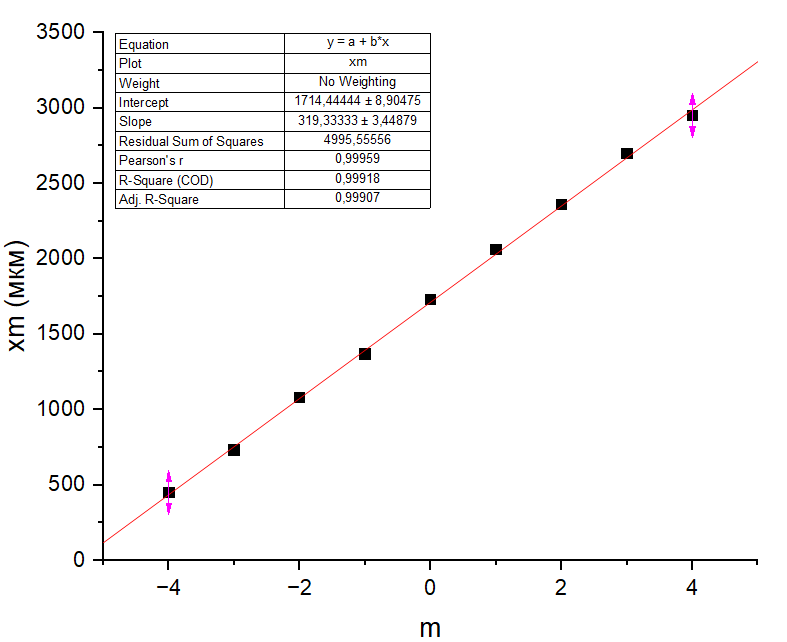
\includegraphics[width=0.65\textwidth]{4.3.2_5.png}\\
\textbf{Рис. 5.} График зависимости координаты $m$-того максимума $x_{m}$ дифракционной картины при частоте генератора $\nu_{1} = 1.17$ МГц \\
\end{center}

$$
\fbox{\nu_{2} = 1.82 \text{ МГц:}}
$$

\begin{center}
\begin{tabular}{|c|c|c|c|c|c|c|c|}\hline
$ m $ & $ -3 $ & $ -2 $ & $ -1 $ & $ 0 $ & $ 1 $ & $ 2 $ & $ 3 $ \\\hline
$ x_{m}, $ мкм & $ 50 $ & $ 460 $ & $ 1150 $ & $ 1590 $ & $ 2110 $ & $ 2710 $ & $ 3280 $ \\\hline
\end{tabular} \\
\hfill \break \textbf {Таблица 2.} Координаты $m$-того максимума $x_{m}$ дифракционной картины при частоте генератора $\nu_2 = 1.82$ МГц \\
\end{center}

\begin{center}
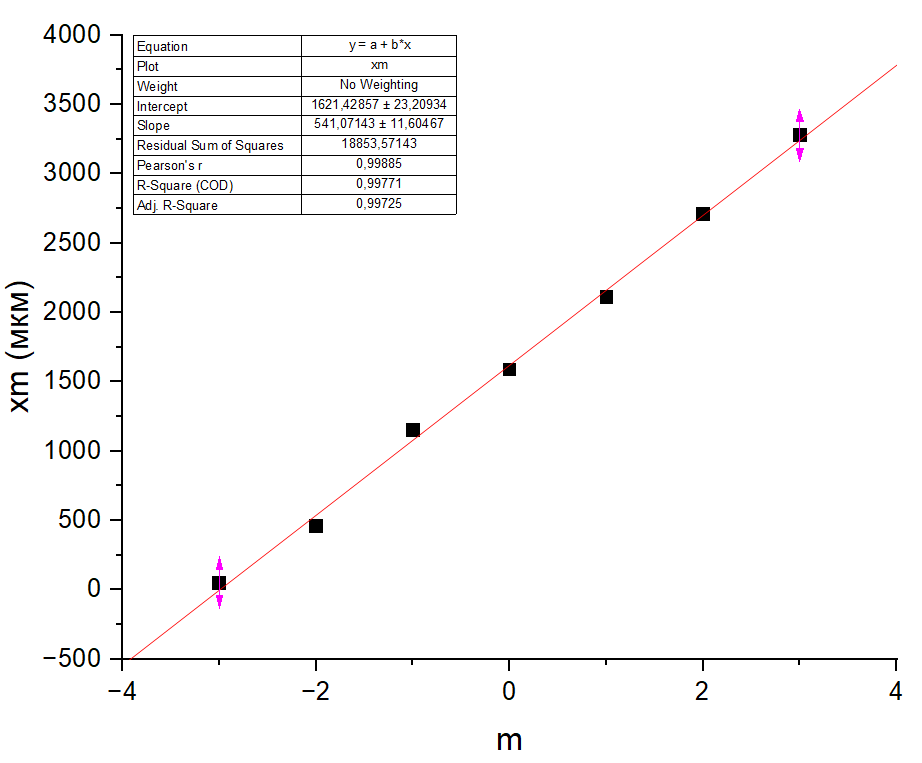
\includegraphics[width=0.65\textwidth]{4.3.2_6.png}\\
\textbf{Рис. 6.} График зависимости координаты $m$-того максимума $x_{m}$ дифракционной картины при частоте генератора $\nu_{2} = 1.82$ МГц \\
\end{center}

$$
\fbox{\nu_{3} = 1.55 \text{ МГц:}}
$$

\begin{center}
\begin{tabular}{|c|c|c|c|c|c|c|c|}\hline
$ m $ & $ -3 $ & $ -2 $ & $ -1 $ & $ 0 $ & $ 1 $ & $ 2 $ & $ 3 $ \\\hline
$ x_{m}, $ мкм & $ 460 $ & $ 790 $ & $ 1230 $ & $ 1610 $ & $ 2030 $ & $ 2540 $ & $ 3000 $ \\\hline
\end{tabular} \\
\hfill \break \textbf {Таблица 3.} Координаты $m$-того максимума $x_{m}$ дифракционной картины при частоте генератора $\nu_3 = 1.55$ МГц \\
\end{center}

\begin{center}
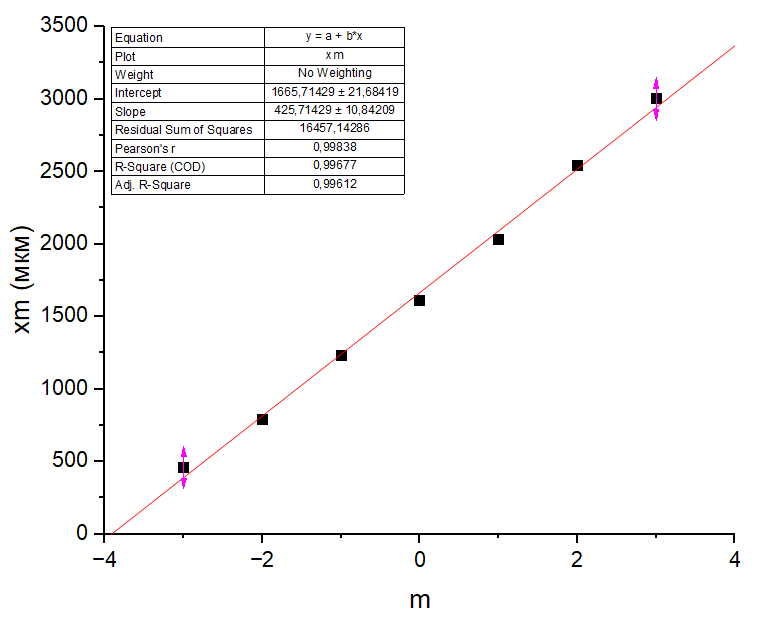
\includegraphics[width=0.65\textwidth]{4.3.2_7.png}\\
\textbf{Рис. 7.} График зависимости координаты $m$-того максимума $x_{m}$ дифракционной картины при частоте генератора $\nu_{3} = 1.55$ МГц \\
\end{center}

$$
\fbox{\nu_{4} = 3.96 \text{ МГц:}}
$$

\begin{center}
\begin{tabular}{|c|c|c|c|c|c|}\hline
$ m $ & $ -2 $ & $ -1 $ & $ 0 $ & $ 1 $ & $ 2 $ \\\hline
$ x_{m}, $ мкм & $ 440 $ & $ 1000 $ & $ 2790 $ & $ 3730 $ & $ 5070 $ \\\hline
\end{tabular} \\
\hfill \break \textbf {Таблица 4.} Координаты $m$-того максимума $x_{m}$ дифракционной картины при частоте генератора $\nu_4 = 3.96$ МГц \\
\end{center}

\begin{center}
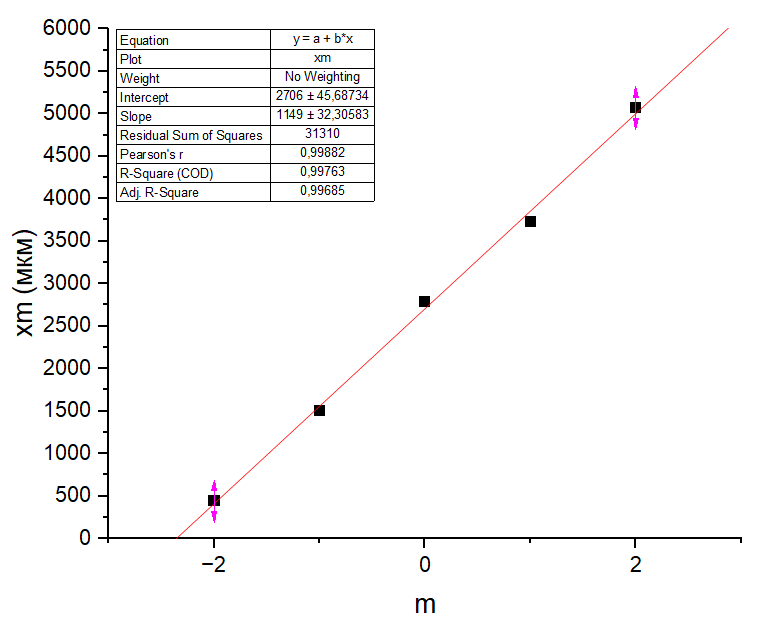
\includegraphics[width=0.65\textwidth]{4.3.2_8.png}\\
\textbf{Рис. 8.} График зависимости координаты $m$-того максимума $x_{m}$ дифракционной картины при частоте генератора $\nu_{4} = 3.96$ МГц \\
\end{center}

\hfill \break По наклону прямой определим расстояние между соседними полосами $l_{m}/m = \Delta x_{m} / \Delta m = k$:

\begin{center}
\begin{tabular}{|c|c|c|c|c|}\hline
$ \text{ } $ & $ \nu_1 $ & $ \nu_2 $ & $ \nu_3 $ & $ \nu_4 $ \\\hline
$ k $, мкм & $ 319.3 \pm 3.4 $ & $ 541.1 \pm 11.6 $ & $ 425.7 \pm 10.8 $ & $ 1149.0 \pm 32.3 $ \\\hline
\end{tabular} \\
\hfill \break \textbf {Таблица 5.} Коэффициенты наклона графиков зависимости максимумов дифракционной картины от их порядков \\
\end{center}

\hfill \break Рассчитаем длину $\Lambda$ УЗ-волны по формуле (6):

$$
l_{m} = mf \frac {\lambda} {\Lambda}, \text{ } \Rightarrow \Lambda = \frac {mf\lambda} {l_{m}} = \frac {f \lambda} {k} \approx (315.4 \pm 96.4) \text{ мкм}.
$$

\hfill \break Определим погрешности рассчитанных величин. 

$$
\sigma_{k_{\text{ср}}} = \sqrt{ \frac {\sum_{i = 1}^{4} (k_{i} - k_{\text{ср}})^2} {12} } = 185.7 \text{ мкм},
$$

\hfill \break где $k_{\text{ср}} = 608.8$ мкм. Тогда $k = 608.8 \pm 185.7$ мкм. При этом $\varepsilon_{\Lambda} = \varepsilon_{k}$.

\hfill \break Также рассчитаем скорость ультразвука в воде по формуле (5):

$$
v = \Lambda \nu = (1513 \pm 35) \text{ м/с}.
$$

\hfill \break Для сравнения табличное значение скорости ультразвуковой волны в воде при комнатной температуре $v_{\text{зв}} = 1490$ м/с.

\subsection{Определение скорости ультразвука методом темного поля}
\hfill \break Для перехода к методу темного поля, не смещая микроскоп, введем микрометрическим винтом в поле зрения микроскопа вертикальную нить (проволочку): резкое изображение нити должно совпадать с резким изображением щели. Не меняя положения отсчетного устройства, отодвинем микроскоп и поставим дополнительную линзу сразу за отсчетным устройством. Опустим в воду пластинку с миллиметровыми делениями и прижмем к задней (по ходу луча) стенке кюветы. Откроем пошире входную щель. С помощью листа бумаги найдем плоскость, в которой располагается резкое изображение линейки, созданное двумя линзами; передвигая микроскоп, сфокусируем его на изображение линейки. Совместим самые дальние из хорошо видимых в поле зрения миллиметровых делений пластинки с делениями окулярной шкалы. Определим цену деления окулярной шкалы в условиях эксперимента через период сетки $h = 1$ мм. $n = 22$ дел/кл, то есть 1 дел $= 45$ мкм. 

\hfill \break Уберем пластинку из кюветы и уменьшим ширину входной щели, включим генератор и попытаемся увидеть звуковую решетку. Уменьшая мощность излучателя, добьемся исчезновения видимого изображения решетки в поле зрения микроскопа. Закроем центральный дифракционный максимум вертикальной нитью. Удобно устанавливать нить в отсутствие УЗ-сигнала, так как в этом случае нет никаких максимумов, кроме нулевого (изображения щели), так что правильно установленная нить должна полностью затемнять поле зрения. 

\hfill \break Включим генератор и найдем изображение акустической решетки. Определим длину УЗ-волны в воде. Для этого с помощью окулярной шкалы измерим расстояние между самыми дальними из хорошо видимых в поле зрения темных (или светлых) полос и просчитаем число промежутков между ними; по формуле $\Lambda = 45$ мкм $\cdot 2 \cdot n/m$ найдем длину ультразвуковой волны $-$ результаты в таблице 6:

\begin{center}
\begin{tabular}{|c|c|c|c|}\hline
$ \nu $, МГц & $ 1.7070 $ & $ 2.0866 $ & $ 4.2673 $ \\\hline
$ n $, дел & $ 65 $ & $ 44 $ & $ 43 $ \\\hline
$ m $, линий & $ 8 $ & $ 7 $ & $ 14 $ \\\hline
$ \Lambda $, мкм & $ 183 $ & $ 142 $ & $ 69 $ \\\hline
\end{tabular} \\
\hfill \break \textbf {Таблица 6.} Результаты измерения длины волны \\
\end{center}

\hfill \break На графике на рис. 9 изобразим график зависимости вида $\Lambda = \Lambda(1/\nu)$ по результатам измерений и расчетов, представленных в таблице 6.

\begin{center}
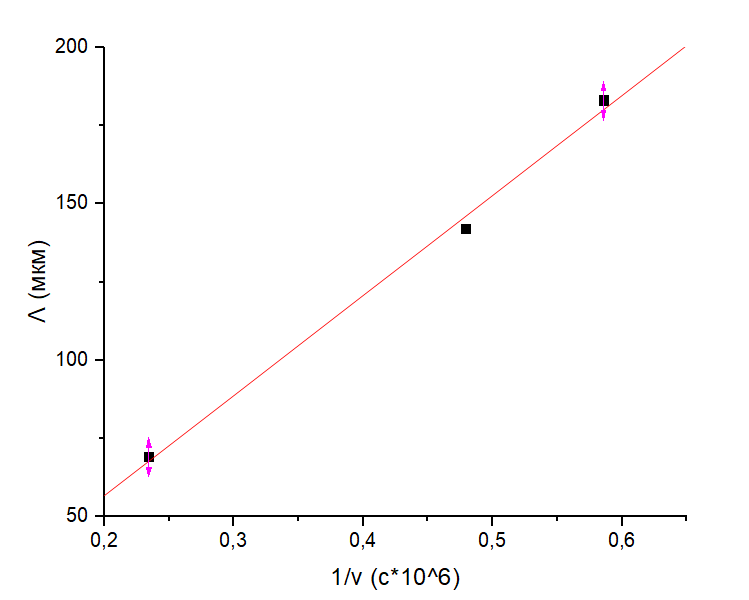
\includegraphics[width=0.75\textwidth]{4.3.2_9.png}\\
\textbf{Рис. 9.} График зависимости длины ультразвуковой волны от $(1/\nu)$ \\
\end{center}

\hfill \break По наклону полученного графика можем определить скорость звука:

$$
v = \Lambda \nu = k = (1419 \pm 40) \text{ м/с}, 
$$

\hfill \break что достаточно близко к табличному значению с учетом погрешности. Инструментальные погрешности малы по сравнению с погрешностями, следующими из МНК, поэтому учитываем только последние. 

\hfill \break Наконец, закрывая ненулевые максимумы, получаем равномерную засветку, так как интенсивность нулевого максимума многократно превышает интенсивность ненулевых. 

\section{Вывод}
\hfill \break Была изучена дифракция света на синусоидальной акустической решетке, рассчитаны длина ультразвуковой волны и скорость ее распространения в воде, которая почти совпала с табличным значением; был применен и изучен метод темного поля в наблюдении фазовых объектов.

\end{document}
